\documentclass[journal,12pt,twocolumn]{IEEEtran}


\usepackage{amsmath,amssymb,amsthm}
\usepackage{graphicx}
\graphicspath{{figs/}}

\begin{document}
	\vspace{3cm}
	\title{ASSIGNMENT 1}
	\author{Prabhav Singh- BT21BTECH11004}
	
	\maketitle
	\textbf{PROBLEM 9(b)}:-Using Properties of proportion solve for x, given\\
	
	
	\hspace*{2cm}$ 	\dfrac{\sqrt{5x}+\sqrt{2x-6}}{\sqrt{5x}-\sqrt{2x-6}} =4 $
	
	
	\medskip
	
	
	\textbf{SOLUTION}:-\\
	Using Componendo and Dividendo rule that is if $  \frac{a}{b} =\frac{c}{d} \implies \frac{a+b}{a-b} =\frac{c+d}{c-d}; $ on the given expression\\
	
	 $	\dfrac{\sqrt{5x}+\sqrt{2x-6}}{\sqrt{5x}-\sqrt{2x-6}} =\dfrac{4}{1} $
	
	\begin{align}
		\dfrac{\sqrt{5x}+\sqrt{2x-6}+\sqrt{5x}-\sqrt{2x-6}}{\sqrt{5x}+\sqrt{2x-6}-\sqrt{5x}+\sqrt{2x-6}} =\dfrac{4+1}{4-1} \\ 
		\dfrac{2\sqrt{5x}}{2\sqrt{2x-6}} =\dfrac{5}{3} \\
		3(\sqrt{5x})=5(\sqrt{2x-6}) \\
		9\times5x=5\times5\times(2x-6) \\
		\ 9x=10x-30 \\
		\implies \boxed{ x=30} 
	\end{align}
	
	\medskip
	
	\begin{figure}[h]
		\centering
		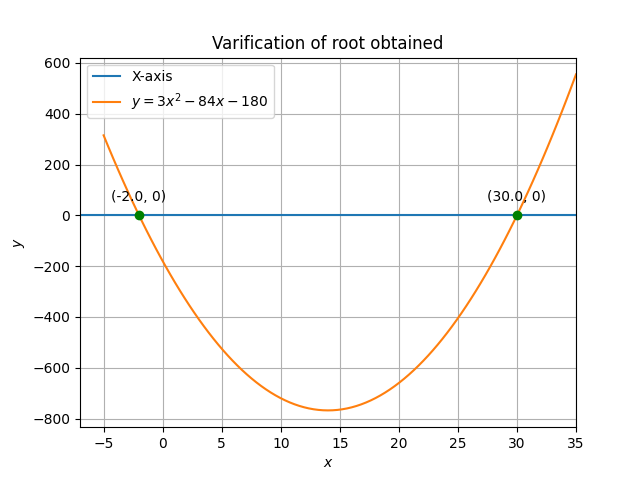
\includegraphics[width=\columnwidth]{output2.png}
		\caption{Zeroes of $ f(x) = 0 $ are intersections of $ f(x) $ with $x-axis $}
		\label{Fig1}
	\end{figure}

	In order to varify the solution using graph we can reduce the given form into a polynomial form by rationalization and squaring .By doing these operations along with simplification we get a quaderatic equation 
	\begin{equation}
		3x^{2}-84x-180=0
	\end{equation}
whose roots are $ -2 $ and $ 30 $ as the graph cuts $  x- axis(y=0  $ line) at $  x= -2 $ and $ x=30 $. But since we have squared the original equation ,so one extra root which is$  x= -2  $,we are getting. Also one can see the domain of original equation is$  [3,\infty] $ since the value inside square root cannot be negative real number. 


	Since at $ x=30 $ the graph cuts the $ x-axis \implies x=30 $ is solution for given equation.
\end{document}
